 %!TEX root = ./template-skripsi.tex
%-------------------------------------------------------------------------------
%                            BAB II
%               KAJIAN TEORI
%-------------------------------------------------------------------------------

\chapter{KAJIAN PUSTAKA}

\section{Proses \emph{Indexing}}

\emph{Indexing} adalah proses pemetaan seluruh data pada \emph{database}.
Proses dimulai dengan mengambil data mentah dari \emph{repository}, yaitu tempat
penampungan data yang telah dikumpulkan oleh \emph{crawler}. Data tersebut
kemudian akan dipetakan sesuai dengan struktur index yang digunakan. Hasil dari
proses indexing adalah sebuah daftar \emph{index}, yang memiliki cara kerja yang
serupa dengan index yang biasa ditemui pada bagian belakang sebuah buku. Index
adalah suatu representasi data yang merujuk kepada lokasi data yang lebih
lengkap di dalam database.

Index merupakan komponen penting dalam suatu arsitektur mesin pencari.
Penggunaan index memberikan pengaruh signifikan dalam proses penerimaan data
dari database karena dapat mengurangi waktu akses \emph{storage}. Hal ini
sejalan dengan pola penggunaan mesin pencari, dimana mayoritas operasi yang
dilakukan adalah memberikan informasi berdasarkan \emph{query} dari pengguna.
Selain itu, representasi index tertentu juga dapat mempengaruhi pengolahan
\emph{query}, penggunaan ruang pada media penyimpanan dan akurasi dari hasil
\emph{query} tersebut.

% TODO Verif ke pak Eka apakah ini masih perlu atau tidak
% Terkait apakah database yang dibutuhkan adalah untuk full-text
Database yang digunakan oleh mesin pencari adalah database yang dirancang
untuk kebutuhan penyimpanan teks secara penuh. Untuk keperluan tersebut,
setidaknya terdapat tiga syarat yang perlu dipenuhi ketika ingin menentukan
representasi index.

\begin{enumerate}
  \item{Memungkinkan untuk mendapatkan data berdasarkan suatu query}

  Dari suatu query pencarian, database harus dapat memberikan hasil yang dapat
  memenuhi query tersebut. Pada konteks penerimaan data yang berbentuk teks,
  konjungsi query sangat umum digunakan. Dalam kasus ini, index harus mampu
  memberikan informasi apakah suatu \emph{record} mengandung kata tertentu, dan
  secara langsung mempengaruhi penentuan granularitas index.

  \item{Menambahkan \emph{record} baru secara efisien}

  Database yang hanya menyimpan teks umumnya digunakan untuk keperluan
  penyimpanan. Pada kasus mesin pencari, operasi yang sering dilakukan adalah
  penulisan data dari \emph{crawler} ke database dan pembacaan data berdasarkan
  query. Operasi untuk mengubah atau menghapus data jarang diperlukan, walaupun
  operasi tersebut tetap perlu didukung.

  \item{Memberikan skor terhadap hasil dari query yang bersifat `informal'}

  Pada kasus mesin pencari, pengguna seringkali memberikan query yang bersifat
  `informal', yaitu query yang tidak dapat dipenuhi seluruhnya oleh database.
  Dalam hal ini, database perlu memberikan hasil yang paling mendekati
  ekspektasi dari query tersebut dengan cara menyertakan nilai relevansi suatu
  data terhadap query.

  Mesin pencari setidaknya membutuhkan syarat pertama dan kedua untuk dipenuhi
  oleh database agar dapat digunakan di dunia nyata.

\end{enumerate}

\section{\emph{Repository}}

\emph{Repository} merupakan tempat penyimpanan seluruh kode HTML dari setiap
halaman web yang telah di-\emph{crawl}. Setiap dokumen memiliki data tambahan
yang disematkan kepadanya, yaitu nomor \emph{id} yang dibuatkan untuk dokumen
tersebut, panjang dari dokumen, dan \emph{URL} dari dokumen tersebut. Seluruh
data tersebut dikompres dengan library \emph{zlib} untuk mengurangi penggunaan
ruang pada \emph{repository}.

\section{Daftar URL}

Ketika mengolah data dari \emph{repository}, terdapat langkah tambahan yang
dilakukan jika menemui \emph{anchor text}. \emph{Anchor text} adalah teks berupa
URL yang merujuk kepada dokumen lain. Setiap \emph{anchor text} yang ditemukan
pada data dari \emph{repository} akan disimpan pada sebuah daftar URL\@.

\section{\emph{Document Index}}
\emph{Document index} menyimpan beberapa informasi tambahan pada setiap dokumen.
Setiap index akan memiliki nomor dokumen, status dokumen, alamat tempat dokumen
tersimpan di \emph{repository}, dan \emph{checksum}. Apabila pada suatu dokumen
telah dilakukan proses \emph{crawling}, maka akan disematkan data tambahan yang
berisi sepasang informasi berupa URL dan judul dari dokumen tersebut. Jika
belum melalui tahap \emph{crawling}, maka data tambahan tersebut hanya merujuk
kepada URL yang terdapat pada daftar URL\@.

\section{Daftar Kosakata}

Setiap hasil pengolahan data dari \emph{repository} akan memberikan daftar
kosakata yang bersifat unik. Daftar kosakata tersebut kemudian akan digabungkan
kedalam daftar kosakata yang menampung keseluruhan kosakata pada database yang
telah melalui proses \emph{indexing}.

Implementasi daftar kosakata ini terbagi menjadi dua bagian, yaitu daftar
kosakata itu sendiri dan daftar \emph{pointer} yang merujuk kepada dokumen
tempat kosakata itu berada. Selain itu, daftar kosakata dapat menyematkan
informasi tambahan seperti jumlah dokumen tempat kosakata tersebut muncul.

Untuk mencegah akses ke ruang penyimpanan yang berlebihan, salah satu syarat
dasar dari implementasi index adalah daftar seluruh kosakata dapat dimuat dalam
memori. Hal ini bertujuan untuk memastikan bahwa dalam situasi pencarian hasil
dengan query boolean, hanya membutuhkan setidaknya satu kali akses ke ruang
penyimpanan per kata.

\section{\emph{Inverted Index}}

\emph{Inverted index} merupakan jenis index yang memetakan potongan isi dari
suatu dokumen atau koleksi dokumen terhadap lokasi aslinya di dokumen atau
koleksi dokumen tersebut. Karena bentuk strukturnya, inverted index cocok
digunakan untuk kebutuhan penerimaan data berdasarkan query seperti mesin
pencari.

% \subsection{Struktur \emph{Inverted File Index}}

% Umumnya, implementasi dari inverted file index terdiri dari dua bagian, yaitu
% suatu struktur pencarian yang berisi seluruh kata pada seluruh dokumen yang
% telah di-\emph{index}, dan daftar dokumen yang telah di-\emph{index} beserta
% informasi lebih dalam terkait keberadaan kata pada struktur pencarian tersebut.

% Clarification
% jangan gunakan istilah struktur pencarian, pecah menjadi kegunaaannya
% masing-masing
% \subsubsection{Struktur Pencarian}
%
% Struktur pencarian terdiri dari dua bagian, yaitu daftar kata yang telah di
% index dan data tentang dokumen tempat kemunculan kata tersebut. Implementasi
% dari inverted file index mengasumsikan jika perangkat memiliki cukup memori
% untuk menampung seluruh struktur pencarian. Hal ini bertujuan untuk memastikan
% bahwa pencarian hasil yang dapat memenuhi suatu query boolean hanya membutuhkan
% setidaknya sekali akses ke ruang penyimpanan per kata.
%
% Akses terhadap ruang penyimpanan perlu dibatasi se minimal mungkin. Hal ini
% berdasarkan contoh kasus penggunaan database untuk kebutuhan mesin pencari.
% Karena jumlah data pada internet yang begitu banyak, proses pemetaan informasi
% dari seluruh internet akan menghasilkan data yang berukuran sangat besar. Hal
% ini akan menyebabkan proses baca ke ruang penyimpanan, walaupun hanya satu kali,
% memakan waktu yang tidak sebentar.

\subsection{Struktur Index}

Representasi dari kemunculan suatu kata pada dokumen, atau biasa disebut sebagai
\emph{hit}, memiliki beberapa data tertentu terkait kata yang dikandung. Setiap
\emph{hit} merepresentasikan suatu kemunculan kata beserta data berikut:

\begin{itemize}
  \item{Lokasi kata dalam dokumen}
  \item{Jenis \emph{font} yang digunakan}
  \item{Informasi terkait penggunaan huruf kapital}
\end{itemize}

\emph{Hit} terbagi menjadi tiga jenis berdasarkan lokasinya dalam struktur
halaman web. Yang pertama adalah \emph{fancy hit}, yaitu \emph{hit} yang berada
didalam \emph{URL}, judul halaman, atau \emph{meta tag}. Yang kedua adalah
\emph{anchor hit}, yaitu \emph{hit} yang khusus berada di dalam
\emph{anchor text} yang merupakan URL yang merujuk kepada dokumen atau halaman
lain. Yang ketiga adalah \emph{plain hit}, yaitu \emph{hit} yang berada diluar
lingkup dari \emph{fancy hit}.

Alokasi memori yang dibutuhkan untuk menyimpan sebuah \emph{hit} adalah 8 byte
atau 16 bit. Penggunaan bit tersebut berbeda tergantung dari jenis \emph{hit},
tetapi memiliki cara yang hampir sama dalam menggunakannya. 

Bit pertama digunakan sebagai penanda untuk penggunaan huruf kapital.
Selanjutnya, bit kedua hingga keempat digunakan sebagai penanda ukuran font yang
digunakan. Ukuran font ini bersifat relatif terhadap seluruh kata dalam dokumen.
Selain itu, nilai bit \emph{111} tidak digunakan sebagai ukuran penanda ukuran
font, namun digunakan sebagai penanda untuk \emph{fancy hit}. Bit kelima hingga
terakhir digunakan sebagai penanda posisi kata dalam dokumen. Karena
keterbatasan bit, posisi yang memiliki nilai lebih dari 4095 akan dianggap
bernilai 4096.

\begin{figure}[H]
  \centering{}
	\includegraphics[width=0.85\textwidth]{gambar/plain\-bit}
  \caption{Penggunaan alokasi memori dari \emph{plain hit}}
\end{figure}

Pada penggunaan \emph{fancy hit}, alokasi bit untuk penanda posisi dibagi
menjadi dua. Bit ke-9 hingga ke-12 digunakan sebagai penanda jenis dari
\emph{fancy hit}, sementara bit ke-13 hingga terakhir tetap digunakan sebagai
penanda posisi.

\begin{figure}[H]
  \centering{}
	\includegraphics[width=0.85\textwidth]{gambar/fancy\-bit}
  \caption{Penggunaan alokasi memori dari \emph{fancy hit}}
\end{figure}

Dari penggunaan \emph{fancy hit}, penggunaan \emph{anchor hit} membagi sisa
delapan bit terakhir menjadi dua, yaitu empat bit awal sebagai penanda posisi
dan empat bit terakhir sebagai nilai \emph{hash} dari dokumen dimana kata
tersebut berada.

\emph{Hit} dirangkai dengan menggunakan struktur \emph{linked list} agar
penambahan hit lebih mudah dilakukan ketika proses indexing ulang. Urutan dari
\emph{hit} dimulai dari kemunculan pertama kata tersebut dalam dokumen tertentu.
\emph{Hit} pertama dalam dokumen kemudian disambungkan ke \emph{id} dari dokumen
di depannya dengan menggunakan pointer.

\begin{figure}[H]
  \centering{}
	
\includegraphics[width=0.85\textwidth]{gambar/linkedListHit}
  \caption{Rangkaian \emph{hit} dengan struktur data \emph{linked list}}
\end{figure}

Iterasi terhadap seluruh \emph{hit} dapat dihindari dengan menyimpan total
\emph{hit} untuk suatu kata dalam suatu dokumen di depan rangkaian \emph{hit}.
Hal ini akan membuat proses penambahan \emph{hit} menjadi lebih efisien dan
memudahkan kalkulasi tingkat kepentingan suatu kata.

\begin{figure}[H]
  \centering{}
	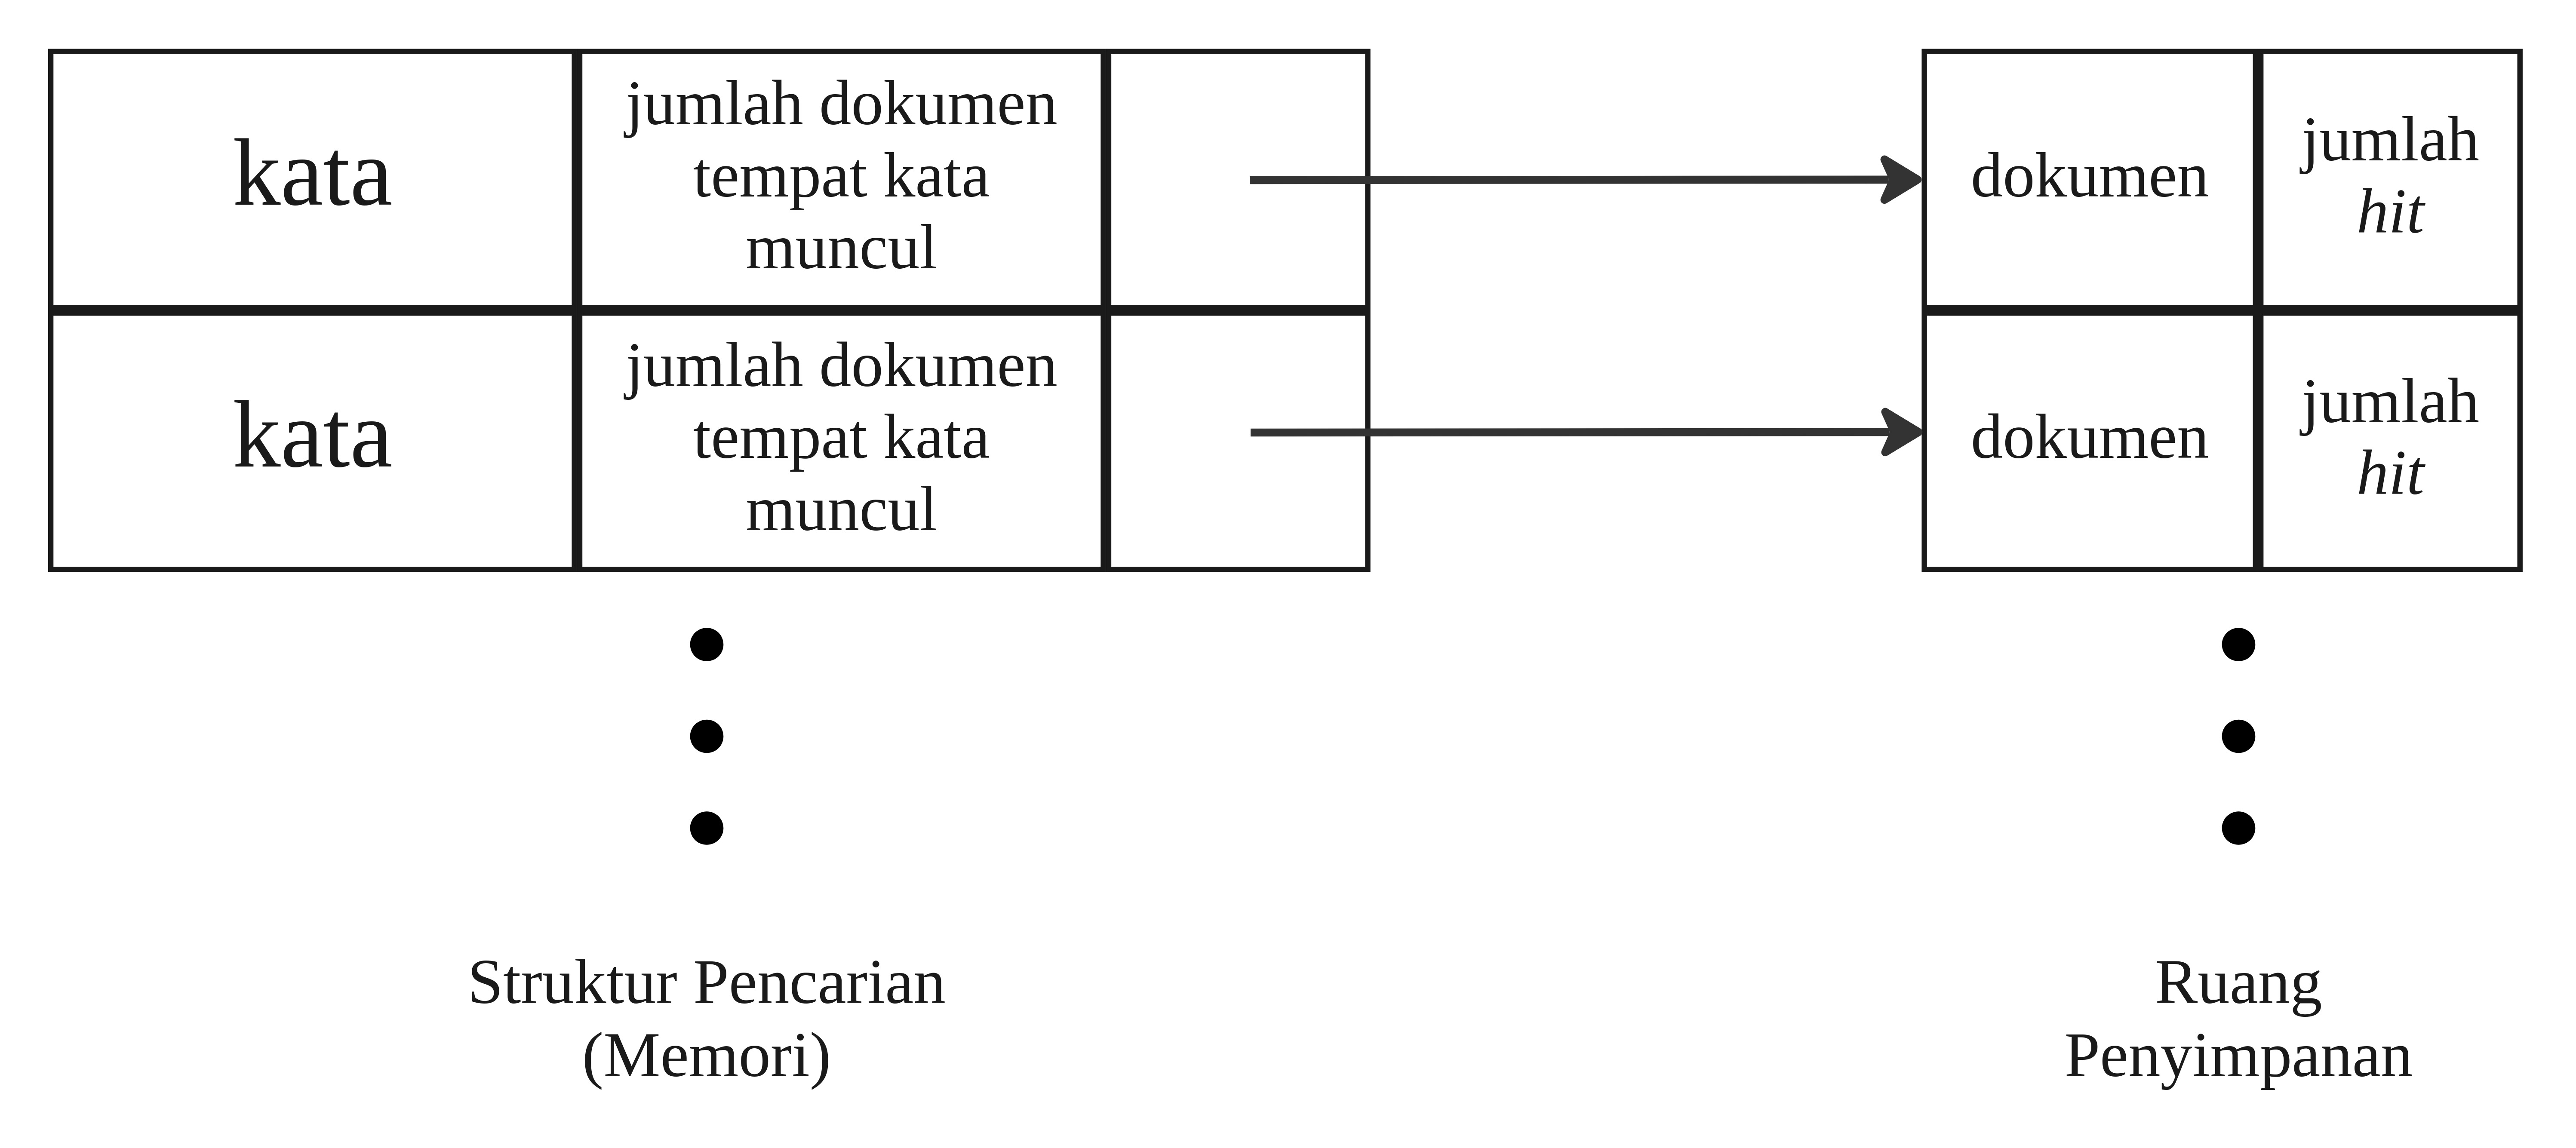
\includegraphics[width=0.85\textwidth]{gambar/hubunganStrukturPencarian}
  \caption{Penempatan jumlah \emph{hit} dalam struktur index}
\end{figure}

\subsection{Skema Penyimpanan Index}

Proses indexing akan menghasilkan \emph{forward index}, yaitu index yang telah
terurut berdasarkan \textit{id} dari dokumen. Untuk membuat \textit{inverted
index}, data pada \textit{forward index} akan diurutkan berdasarkan \textit{id}
dari kosakata.

Kemudian, dibuat dua salinan dari daftar index. Salinan pertama berisi daftar
\emph{hit} yang termasuk dalam kategori \emph{fancy hit} atau \emph{anchor hit}.
Salinan kedua adalah daftar \emph{hit} sisanya. Hal ini bertujuan untuk
mengurangi kemungkinan akses dari index, karena pada sebagian besar kasus query
dapat dipenuhi dengan hanya mengakses data pada \emph{fancy hit} dan
\emph{anchor hit}.

Pada contoh kasus mesin pencari, jumlah data di seluruh internet yang terus
bertambah membuat potensi penggunaan media penyimpanan menjadi hampir tidak
terbatas. Hal tersebut dapat menyebabkan tidak cukupnya kapasitas memori untuk
menampung seluruh index. Untuk mengatasinya, skema penyimpanan index perlu di
partisi menjadi beberapa bagian.

Selain itu, pada tiap salinan index, index juga akan di sortir berdasarkan
\emph{id} dari dokumen. Tujuannya adalah untuk memudahkan proses \emph{merging}
ketika dihadapkan pada situasi dimana query memiliki banyak kata.

% \subsection{Pemeringkatan Query}
%
% Untuk memenuhi kebutuhan tambahan seperti pemeringkatan query, struktur
% pencarian perlu menampung data tambahan seperti frekuensi kemunculan kata dan
% parameter kompresi. Apabila data tersebut tidak dapat dimuat seluruhnya pada
% memori, maka struktur pencarian dapat dipecah dan disimpan sebagian pada ruang
% penyimpanan. Sebagai contoh, kata yang bersifat umum dapat disimpan pada memori
% untuk mengurangi kemungkinan akses ke ruang penyimpanan.

\section{Proses Pembuatan Index}

Sebagai contoh, pada tabel \ref{tab:lirik} digunakan sampel teks berupa lirik
lagu anak-anak. Pada kasus ini, diasumsikan bahwa setiap baris merupakan isi
dari dokumen terpisah.

\begin{center}
  \begin{longtable}{ P{0.15\textwidth{}} P{0.75\textwidth{}}}
  \caption{Contoh teks dari lirik lagu anak-anak} \label{tab:lirik} \\

  % First page header
  \multicolumn{1}{c}{\textbf{Dokumen}} & \multicolumn{1}{c}{\textbf{Teks}} \\ \hline 
  \endfirsthead

  % Next page header
  \multicolumn{2}{c}%
    {{\textbf{\tablename \space{} \thetable{}:} Contoh teks dari lirik lagu anak-anak}} \\
  \multicolumn{1}{c}{\textbf{Dokumen}} & \multicolumn{1}{c}{\textbf{Teks}} \\ \hline 
  \endhead

  % Next page indication footer
  \hline \multicolumn{2}{r}{{Dilanjutkan pada halaman berikutnya}} \\ \hline
  \endfoot

  % Last footer without next page indication
  \hline \hline
  \endlastfoot

    1 & Pease porridge hot, pease porridge cold, \\
    2 & Pease porridge in the pot, \\
    3 & Nine days old. \\
    4 & Some like it hot, some like it cold, \\
    5 & Some like it in the pot, \\
    6 & Nine days old. \\
  \end{longtable}
\end{center}

Seluruh kata dalam seluruh koleksi dokumen kemudian akan diambil jumlah
kemunculannya beserta nomor dokumen tempat kata tersebut ditemukan, dan
dikumpulkan berdasarkan keunikan kata-nya.

\begin{center}
  \begin{longtable}{ P{0.1\textwidth{}} P{0.1\textwidth{}} P{0.25\textwidth{}}}
  \caption{\textit{Inverted file index} dari lirik lagu pada tabel
  \ref{tab:lirik}} \label{tab:file_index} \\

  % First page header
  \multicolumn{1}{c}{\textbf{Nomor}} & \multicolumn{1}{c}{\textbf{Kata}} & \multicolumn{1}{c}{\textbf{Index}} \\ \hline 
  \endfirsthead

  % Next page header
  \multicolumn{3}{c}%
    {{\textbf{\tablename\ \thetable{}:} \textit{Inverted file index} dari lirik lagu pada tabel
    \ref{tab:lirik}}} \\
  \multicolumn{1}{c}{\textbf{Nomor}} & \multicolumn{1}{c}{\textbf{Kata}} & \multicolumn{1}{c}{\textbf{Index}} \\ \hline 
  \endhead

  % Next page indication footer
  \hline \multicolumn{3}{r}{{Dilanjutkan pada halaman berikutnya}} \\ \hline
  \endfoot

  % Last footer without next page indication
  \hline \hline
  \endlastfoot

    1 & cold & $\langle{}2; 1, 4 \rangle{}$ \\
    2 & days & $\langle{}2; 3, 6 \rangle{}$ \\
    3 & hot & $\langle{}2; 1, 4 \rangle{}$ \\
    4 & in & $\langle{}2; 2, 5 \rangle{}$ \\
    5 & it & $\langle{}2; 4, 5 \rangle{}$ \\
    6 & like & $\langle{}2; 4, 5 \rangle{}$ \\
    7 & nine & $\langle{}2; 3, 6 \rangle{}$ \\
    8 & old & $\langle{}2; 3, 6 \rangle{}$ \\
    9 & pease & $\langle{}2; 1, 2 \rangle{}$ \\
    10 & porridge & $\langle{}2; 1, 2 \rangle{}$ \\
    11 & pot & $\langle{}2; 2, 5 \rangle{}$ \\
    12 & some & $\langle{}2; 4, 5 \rangle{}$ \\
    13 & the & $\langle{}2; 2, 5 \rangle{}$ \\
  \end{longtable}
\end{center}

Hasil index pada tabel \ref{tab:file_index} merupakan bentuk
\textit{inverted file index}, yang memetakan kata ke dokumen tempat kemunculan
kata tersebut. Untuk membuat implementasi ulang modul index milik Google, maka
diperlukan index dengan granularitas yang lebih halus. Modul index milik Google
menggunakan \textit{word-level index}, dimana index juga menyimpan posisi kata
dalam dokumen. \textit{Word-level index} dapat mengatasi situasi dimana jumlah
kemunculan suatu kata dalam dokumen lebih dari satu kali.

Dengan mengabaikan detail selain posisi kata dalam dokumen, index pada tabel
\ref{tab:file_index} dapat dikembangkan menjadi seperti berikut

\begin{center}
  \begin{longtable}{ P{0.1\textwidth{}} P{0.1\textwidth{}} P{0.2\textwidth{}}}
    \caption{\textit{Word-level index} dari lirik lagu pada tabel
    \ref{tab:lirik}}
    \label{tab:word_index} \\
    \textbf{Nomor} & \textbf{Kata} & \textbf{Index} \\
    \hline{}
    1 & cold & $\langle{}2; (1;6), (4;8) \rangle{}$ \\
    2 & days & $\langle{}2; (3;2), (6;2) \rangle{}$ \\
    3 & hot & $\langle{}2; (1;3), (4;4) \rangle{}$ \\
    4 & in & $\langle{}2; (2;3), (5;4) \rangle{}$ \\
    5 & it & $\langle{}2; (4;3,7), (5;3) \rangle{}$ \\
    6 & like & $\langle{}2; (4;2,6), (5;2) \rangle{}$ \\
    7 & nine & $\langle{}2; (3;1), (6;1) \rangle{}$ \\
    8 & old & $\langle{}2; (3;3), (6;3) \rangle{}$ \\
    9 & pease & $\langle{}2; (1;1,4), (2;1) \rangle{}$ \\
    10 & porridge & $\langle{}2; (1;2,5), (2;2) \rangle{}$ \\
    11 & pot & $\langle{}2; (2;5), (5;6) \rangle{}$ \\
    12 & some & $\langle{}2; (4;1,5), (5;1) \rangle{}$ \\
    13 & the & $\langle{}2; (2;4), (5;5) \rangle{}$ \\
  \end{longtable}
\end{center}

\subsection{Pengolahan Query}

Untuk query yang hanya mengandung satu kata, hasil bisa langsung didapatkan
dengan melakukan pencarian kosakata yang memenuhi query pada daftar kosakata.
Setelah ditemukan dokumen yang membuat kata yang memenuhi query tersebut diambil
dengan petunjuk dari data yang disematkan pada daftar kosakata.

Query yang melibatkan banyak kata akan memerlukan proses penggabungan hasil dari
kosakata yang sesuai. Sebagai contoh mudahnya, query yang melibatkan banyak kata
dapat digabungkan dengan menggunakan operator logika. Operator \textit{OR} akan
memberikan gabungan dari hasil. Sementara operator \textit{AND} akan memberikan
irisan dari hasil. Jika diberikan query sebagai berikut

\[
  Q_1 \;\textit{AND} \;Q_2 \;\textit{AND} \;\cdots{} \;\textit{AND} \;Q_N
\]

maka dilakukan pencarian untuk setiap dokumen yang mengandung kata yang memenuhi
seluruh rangkaian $Q_1$ hingga $Q_n$. Dari seluruh dokumen yang sesuai, maka
dicari irisan dari hasil tersebut (dokumen yang memiliki kedua query tersebut).

Sebagai contoh, dari index pada tabel \ref{tab:file_index}, apabila diberikan
query

\[
  hot\; \textit{AND} \;like
\]

maka akan didapatkan lokasi dari index dengan kosakata \textit{hot} dan
\textit{like}, yaitu $\langle{}1, 4 \rangle{}$ dan $\langle{}4, 5 \rangle{}$.
Dari data lokasi tersebut, mereka kemudian digabungkan (diambil irisannya),
sehingga didapatkan dokumen 4 yang memenuhi kedua query tersebut.

Untuk query yang mengandung banyak kata yang tidak digabungkan dengan operator
boolean, penggunaan \textit{inverted file} seperti contoh diatas akan
menimbulkan banyaknya \textit{false match} yang mengurangi kualitas hasil dari
query. \textit{False match} sendiri dapat diatas dengan melakukan pemindaian
untuk memastikan hasil dari query. Tetapi pemindaian akan mengurangi performa
keseluruhan dari proses pengambilan data.

Penggunaan \textit{word-level index} dapat menangani hal tersebut dengan
menggunakan informasi yang lebih lengkap yang tersemat pada tiap \textit{hit}.
Karena terdapat informasi terkait posisi kata dalam dokumen, jarak antara kata
dapat dibandingkan sesuai dengan query.

% \subsection{Query Multi Kata}
%
% Apabila query memiliki lebih dari satu kata, untuk memperoleh hasil yang lebih
% akurat, struktur pencarian membutuhkan data tambahan. Data tersebut adalah
% posisi kata dalam suatu dokumen. Dengan menyimpan posisi kata, dapat dilakukan
% perbandingan posisi antar kata yang terdapat pada query.

\section{Perbandingan Metode \emph{Indexing}}

\subsection{\emph{Signature File Index}}

\emph{Signature file} adalah suatu metode probabilistik yang digunakan sebagai
alternatif untuk mengindeks teks. Pada implementasi \emph{signature file},
setiap dokumen memiliki suatu \emph{descriptor}, yaitu rangkaian \emph{bit} yang
merepresentasikan konten dari dokumen. \emph{Descriptor} dibuat dengan cara
menggunakan beberapa \emph{hash function} untuk mendapatkan suatu rangkaian bit
unik yang merepresentasikan suatu kata dalam dokumen. 

Karena sifatnya yang probabilistik, \emph{descriptor} tidak dapat bersifat unik
sepenuhnya. Terdapat kemungkinan konflik antara \emph{descriptor} dari tiap
kata. Oleh karena itu, setiap hasil \emph{hashing} dari suatu kata yang sesuai
dengan \emph{descriptor} tertentu perlu diartikan sebagai suatu kemungkinan,
bukan suatu kepastian.

Untuk memastikannya, perlu dilakukan \emph{scanning} pada dokumen yang diduga
mengandung kata tersebut. Kemungkinan terjadinya konflik dapat dikurangi dengan
menggunakan lebih banyak bit, tetapi proses \emph{scanning} tetap perlu
dilakukan untuk memastikan ada atau tidaknya suatu kata.

% Signature vs Inverted
Dibandingkan dengan inverted file, signature file memiliki dua kekurangan yang
memiliki dampak langsung untuk kebutuhan mesin pencari. Yang pertama adalah
performa yang lebih lambat dalam hal pengambilan data dari database. Hal ini
dikarenakan perlunya melakukan \emph{scanning} untuk memastikan suatu kata ada
di dalam suatu dokumen. Yang kedua adalah perlunya proses yang rumit untuk
mengolah query yang mengandung disjungsi atau negasi.

Signature file memiliki satu keunggulan dibandingkan inverted file, yaitu tidak
membutuhkan penyimpanan daftar kosakata pada memori. Oleh karena itu, di masa
lalu signature file lebih umum digunakan karena alasa keterbatasan ruang
penyimpanan. Tetapi seiring berjalannya waktu, inverted file mengadopsi teknik
kompresi yang membuat keunggulan signature file ini menjadi tidak berlaku lagi.

\subsection{\emph{Bitmap Index}}

\emph{Bitmap} adalah. Bitmap menggunakan \emph{bitvector} sebagai representasi
index. Setiap kata memiliki \emph{bitvector} yang menunjukkan keberadaan kata
tersebut dalam berbagai dokumen. Panjang dari \emph{bitvector} tergantung dari
jumlah dokumen secara kesuluruhan. Konsep bitmap sangat mudah dan cepat untuk
digunakan. Tetapi, bentuk struktur \emph{bitvector} membuat kebutuhan ruang
penyimpanan menjadi sangat besar.

Karena kekurangannya dalam hal ukuran struktur data, bitmap tidak dapat
digunakan pada berbagai kebutuhan dunia nyata, terutama mesin pencari.

\subsection{\emph{WordNet}}

\emph{WordNet} adalah suatu \emph{synonym ring} yang mampu mengelompokkan kata
berdasarkan makna yang ekuivalen secara semantik (sama secara makna).
\emph{WordNet} dapat digunakan pada proses indexing dengan harapan hasil dari
pengelompokan kata yang ditemukan dalam dokumen dapat menjadi lebih baik. Hal
ini dapat memberikan peningkatan performa dalam proses pengambilan data.

Implementasi index menggunakan \emph{WordNet} dapat digunakan sebagai pembanding
untuk metode \emph{inverted file} yang telah dijelaskan sebelumnya.

\section{Modul $typing$ pada \textit{Python}}

Untuk penjabaran struktur data pada modul \textit{indexing}, penulis menggunakan
bahasa pemrograman \textit{Python}. \textit{Python} dipilih karena seluruh kode
program yang ada pada arsitektur \textit{Telusuri} menggunakan bahasa yang sama.
Selain itu penulis menggunakan modul $typing$ yang mulai diperkenalkan pada
\textit{Python} versi $3.5$ untuk memberikan keterangan yang lebih jelas terkait
tipe data apa yang digunakan.
